%
%
%

\chapter{Introduction to Scilab}

\section{Problem Statement and Learning Objectives}

This chapter will briefly introduce Scilab.  The student should be able to 
\begin{itemize}
    \item Download and install Scilab
    \item Perform basic command line computations including:
    \begin{itemize}
        \item enter a transfer function using {\tt syslin('c', num, den)}.
        \item Generate Bode and Root Locus Plots
        \item Correct the axis scales on plots to increase quality and readability of 
        graphics plots. 
    \end{itemize}
\end{itemize}


\section{Quick Read}
Scilab is an open source numerical computing environment very similar to Matlab.  The cool thing
 about Scilab is that it is 100\% free and you may install it on Windows, Mac, or Linux, it is very powerful, 
 and very similar to Matlab.   If you are comfortable with Matlab, you will easily adapt to Scilab. 

\section{Basics}
Scilab has a multi-windowed interface similar to Matlab.  Once you launch Scilab, you can define variables and 
execute commands in a similar way.  Here is a screen capture of a basic example:

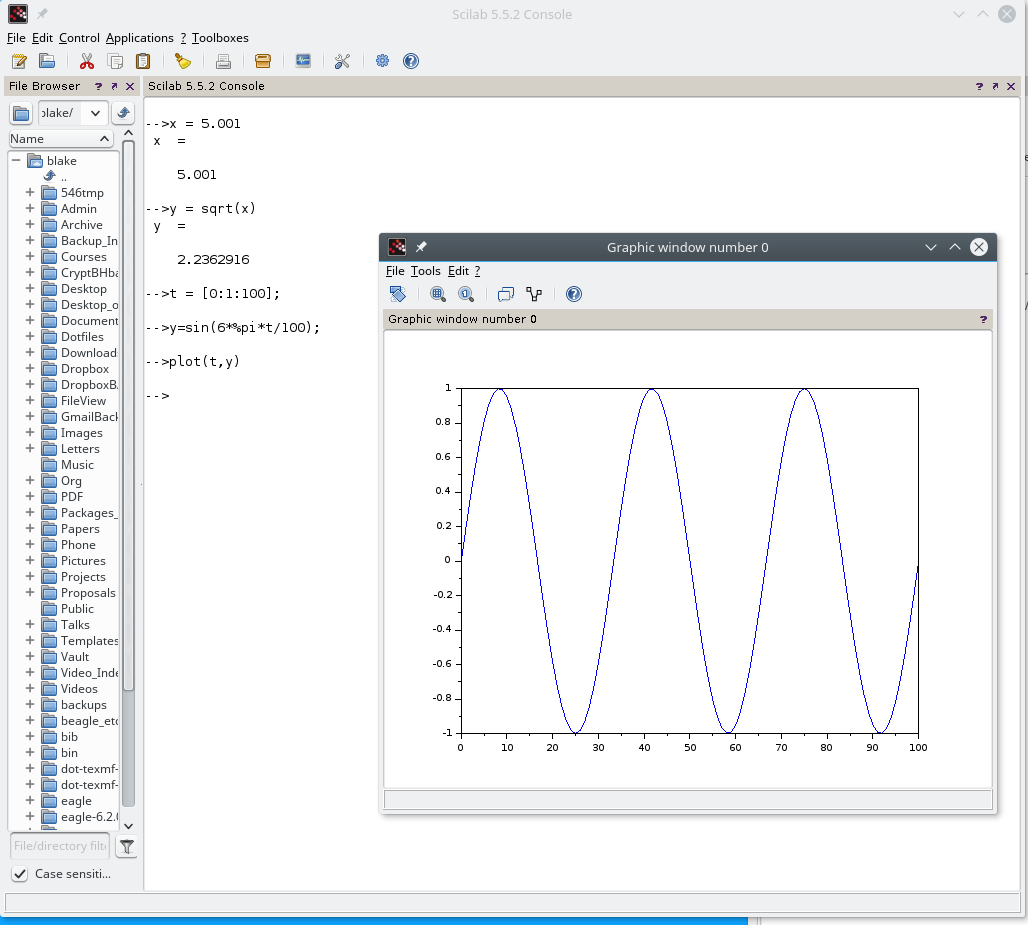
\includegraphics[width=5.5in]{figs08/sshot01.png}

An editor called SciNotes can edit your Scilab scripts (.sce files) and works well. 

\section{Links and details}
For download and detailed documentation, please see

\url{http://www.scilab.org}

\url{http://forge.scilab.org/index.php/p/docintrotoscilab/downloads/311/}

This document, while a bit dated, is geared to transitioning you from Matlab to Scilab: \url{https://wiki.scilab.org/Tutorials?action=AttachFile&do=get&target=Scilab4Matlab.pdf}

 
\section{Root Locus Example}

Let's do the Root locus plot of Example 6.8.  The open loop gain is:
\[
G(s) = C(s)P(s) = \frac {K(s+4)(s+5)} {(s+1+3j)(s+1-3j)}
\]

We'll enter a script to do this in SciNotes:

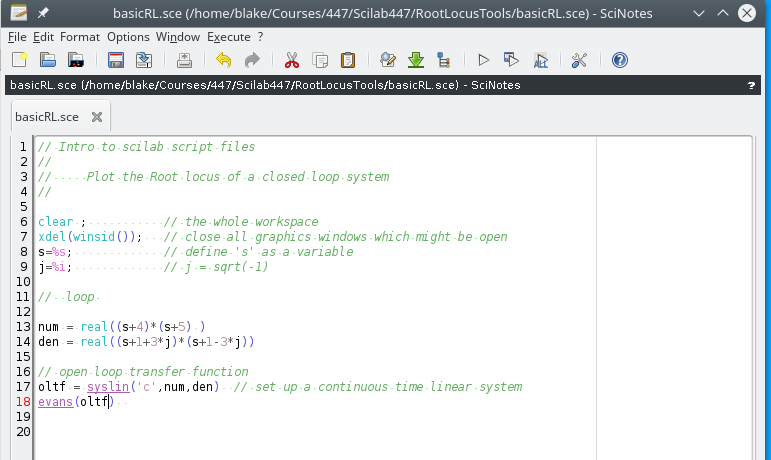
\includegraphics[width=5.5in]{figs08/sshot02.png}

Lines 13 and 14 define the numerator and denominator of the open loop transfer function (loop gain).
We set up the transfer function as a linear system object using the {\tt syslin()} function. 
 {\tt evans()} is the root locus function, so named because of its original inventor Walter Evans. 
We have
added the {\tt real()} operator because the complex conjugate poles cause 
a {\tt +0j} term which confuses {\tt evans()} (Root locus requires real-valued polynomial coefficients). 

The resulting plot is

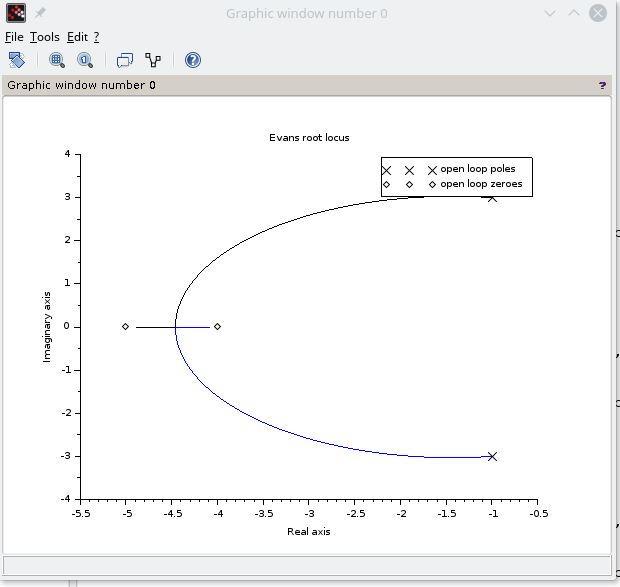
\includegraphics[width=4.0in]{figs08/sshot03.png}

\section{Plotting Ranges for high quality graphics}
Sometimes autoranges provided by graphing software do not result in a graph which shows the desired features. 

In Scilab, we can take control of the plotting axis ranges (as well as many other details) by 
a two step process:
\begin{enumerate}
    \item obtain a pointer or handle to the axes
    \item setting new manually defined axis limits
\end{enumerate}

\begin{Example}
The following is a plot of a polynomial function ($y=-20x+x^2-0.007x^3$). 

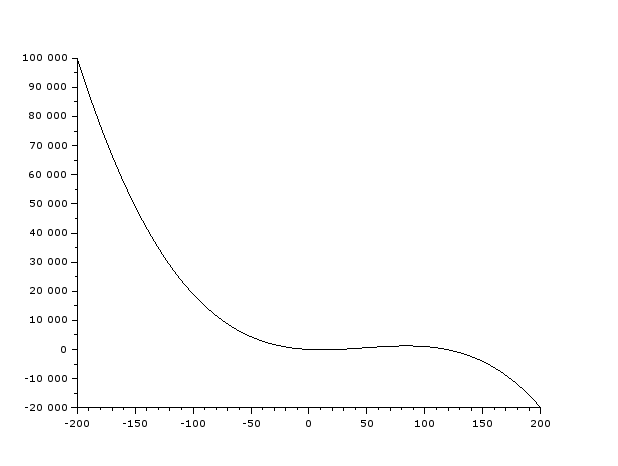
\includegraphics[width=4.0in]{figs08/polynom_01.png}

We are only 
interested in the region for positive x.  Replot this function for the ranges:
\[
0 < x < 200 \qquad -20,000 < y < 10,000
\]
Oh, and by the way, make the plot background yellow!

Solution:

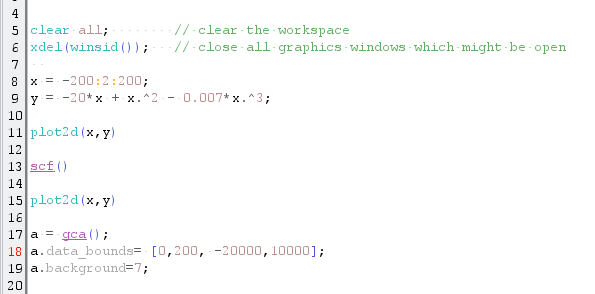
\includegraphics[width=4.5in]{figs08/poly_plot_script.png}


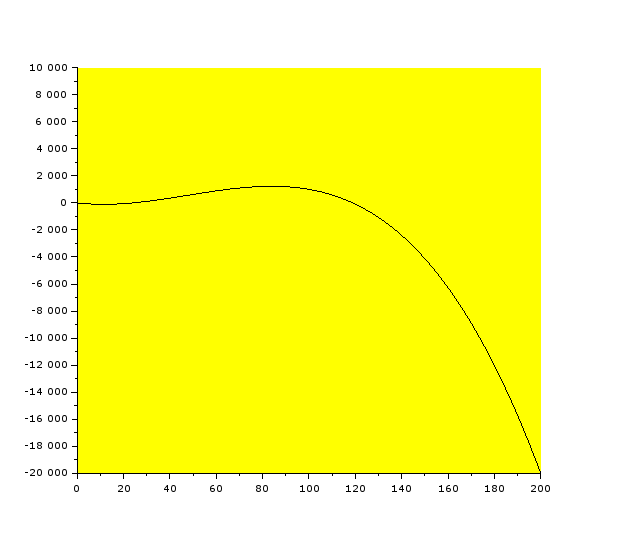
\includegraphics[width=4.0in]{figs08/polynom_02.png}


\end{Example}
All the things you can do to modify plots are documented in the Scilab help system. 

% \section{Summary of Notation}

